\section{Problem 3}
\label{Problem3}

\subsection{Question}
\vspace*{10pt}
Consider the "bow-tie" graph in the Broder et al. paper (fig 9):\\ http://www9.org/w9cdrom/160/160.html\\
\\
Now consider the following graph:
\\
\begin{tabular}{c c c}
A & $\to$ & B\\
B & $\to$ & C\\
C & $\to$ & D\\
C & $\to$ & A\\
C & $\to$ & G\\
E & $\to$ & F\\
G & $\to$ & C\\
G & $\to$ & H\\
I & $\to$ & H\\
I & $\to$ & J\\
I & $\to$ & K\\
J & $\to$ & D\\
L & $\to$ & D\\
M & $\to$ & A\\
M & $\to$ & N\\
N & $\to$ & D\\
O & $\to$ & A\\
P & $\to$ & G\\
\end{tabular}
\vspace*{5mm}

	For the above graph, give the values for:\\
	
	\begin{tabular}{l}
	\textbf{IN}:\\
	\textbf{SCC}:\\
	\textbf{OUT}:\\
	\textbf{Tendrils}:\\
	\textbf{Tubes}:\\
	\textbf{Disconnected}:\\
	
	\end{tabular}
	
\newpage
\vspace*{5pt}
\subsection{Answer}
\begin{center}
	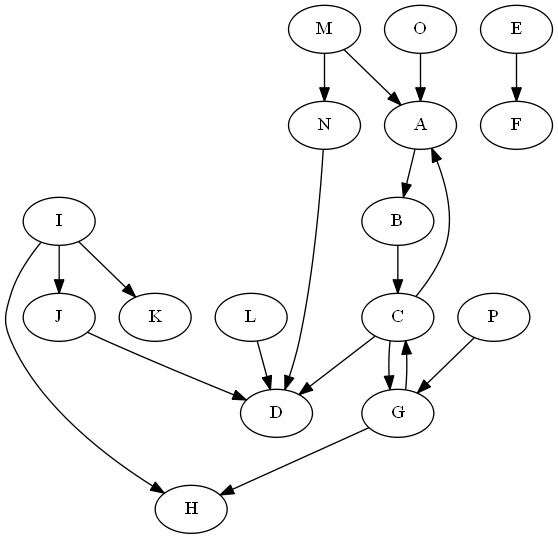
\includegraphics[scale=0.75]{Q3/fig1.png}\\
	\centerline{\textit{Figure 9: Drawing of example graph}}
\end{center}

\textit{Figure 9:} is a \enquote{"bow\-tie"}\cite{bow-tie} graph of the included points, generated using Graphviz\cite{graph}. 

\vspace{5mm}
\begin{tabular}{l l}
	\textbf{IN}: \{\textsc{M,O,P}\} & \enquote{Connects into SCC, but not out from SCC}\\
	\\
	\textbf{SCC}: \{\textsc{A,B,C,G}\} &\enquote{SCC -- all contained nodes are interconnected}\\
	\\
	\textbf{OUT}: \{\textsc{D,H}\} & \enquote{Connects out from SCC, but not in to SCC}\\
	\\
	\textbf{Tendrils}: \{\textsc{I,J,K,L}\} & \enquote{In or out excluding all SCC}\\
	\\
	\textbf{Tubes}: \{\textsc{N}\}& \enquote{IN $\to$ OUT or OUT $\to$ IN connection}\\
	\\
	\textbf{Disconnected}:\{\textsc{E,F}\} & \enquote{Not connected to other sites}\\
\end{tabular}
\\
\vspace{5mm}
The descriptions of each node is a matter of interpretation.  Explanations have been provided for each value assignment.

\textbf{IN:}  $M,O,P$

The IN components form the starting point for connection to the SCC\cite{broder2000}.  They all sit at the start of the graph.  In this graph, because of how the SCC and tubes are defined, the only IN components are $M,O,P$.

\textbf{SCC:}  $A, B, C, G$

The Strongly Connected Component consists of those heavily linked items connected to from the list of nodes listed as part of IN\cite{broder2000}.  It's an $A, B, C, G$ world.

\textbf{OUT:}  $D,H$

The OUT components exit the SCC, but do not link back to it\cite{broder2000}.  The only members of OUT are $D,H$, who forms a sink from members of the SCC and the tendrils.

\textbf{Tendrils:}  $I, J, K, L$

The \emph{Tendrils} are pages that cannot reach the SCC or are not reached from the SCC\cite{broder2000}.  The tendrils come from other graphs and only join the whole via $D or H$.

\textbf{Tubes:} $N$

Then there are \emph{tubes}, which pass from IN to OUT without going through SCC\cite{broder2000}.  $N$ is a tube linking from $M$ (from IN) to $D or H$ (from OUT).

\textbf{Disconnected:}  $E, F$

The Disconnected components link to no one in the graph, and stand alone.  They are not defined explicitly by Broder, et. al, but their meaning is implied within the paper.

